% !TeX spellcheck = en_GB
\documentclass{article}
\usepackage{graphicx}
\usepackage{titlesec}
\usepackage{array}
\usepackage[table]{xcolor}
\usepackage{color, colortbl}
\usepackage{stackengine}
\usepackage{fancyhdr}
\usepackage{longtable}
\usepackage{changepage}
\usepackage{tikz, graphicx}
\usepackage{hyperref}
\usepackage{listings}
\usepackage{float}

\newcommand\xrowht[2][0]
{\addstackgap[.5\dimexpr#2\relax]{\vphantom{#1}}}

\setlength{\arrayrulewidth}{0.4mm}
\setlength{\tabcolsep}{20pt}
\renewcommand{\arraystretch}{1.6}
\setcounter{tocdepth}{4}
\setcounter{secnumdepth}{4}

\pagestyle{fancy}
\renewcommand{\headrulewidth}{2pt}
\renewcommand{\footrulewidth}{1pt}

\begin{document}
\begin{titlepage}
	\begin{center}
		\begin{figure}
			\centering
			
\includegraphics[scale=0.3]{LogoPolimi.PNG} \\
			[0.3cm]
		\end{figure}
		\Huge{\bfseries - DD -} \\
		[0.5cm]
		\huge{Design Document} \\
		[1mm]
		\rule{300pt}{3pt} \\
		[1.0cm]
		\textsc{\Large Computer Science and Engineering} \\ 
		\textsc{\Huge Software Engineering II} \\
		\textsc{\Large A.A. 2020/2021} \\
		[1cm]
		\textsc{\LARGE Daniele Mammone - 10625264} \\
		\textsc{\LARGE Gianmarco Naro - 10610374} \\
		\textsc{\LARGE Massimo Parisi - 10583470} \\
	\end{center}
\end{titlepage}

\newpage

\renewcommand\contentsname{Contents}
\tableofcontents

\newpage

\section{Introduction}

	\subsection{Purpose}
	test
	\subsection{Scope}
	\subsection{Definitions, Acronyms, Abbreviations}
	\subsection{Revision History}
	\subsection{Reference Documents}
	\subsection{Document Structure}

\section{Architectural Design}
	The aim of this section is to give a look to the architectural aspect of the analysed system. In doing this, a top-down approach will be followed, starting from a very general view of the system, then going into more detail through Component Diagrams, more and more detailed. This allows us to precisely describe each component of CLup, so that who will develop the system, well know the behaviour of each component.
	
	
	\subsection{Overview}
	A first high level overview can be done through the system's \textbf{Composition Diagram}. In fact, here there is a first subdivision of the system's component, each one with a different task.
	\begin{itemize}
		\item \textbf{Communication Interfaces}: to work properly, the system needs to interface overt the network with both remote applications, and external services. Because of this, there are some components devoted to interact with remote devices:
		\begin{itemize}
			\item{\bfseries UserHandler}: to interact with users, both Managers and Customers, the latter both at Totems, and on app;
			\item{\bfseries EntranceManagement}: so that the Store can process a scanned QR Code at entry/exit;
			\item{\bfseries NumberCallingInterface}: to notify the call of a certain number;
		\end{itemize}
		and others deputy to access external services, such as 
		\begin{itemize}
			\item{\bfseries Map Component}: to access an external Map Provider
			\item{\bfseries Notification Component}: to send notifications to Customers through an external Notification service 
			\item{\bfseries Mail Component}: to externally sending Mails, avoiding building an internal Mail manager
		\end{itemize}
	\begin{figure}[!h]
		\centering
		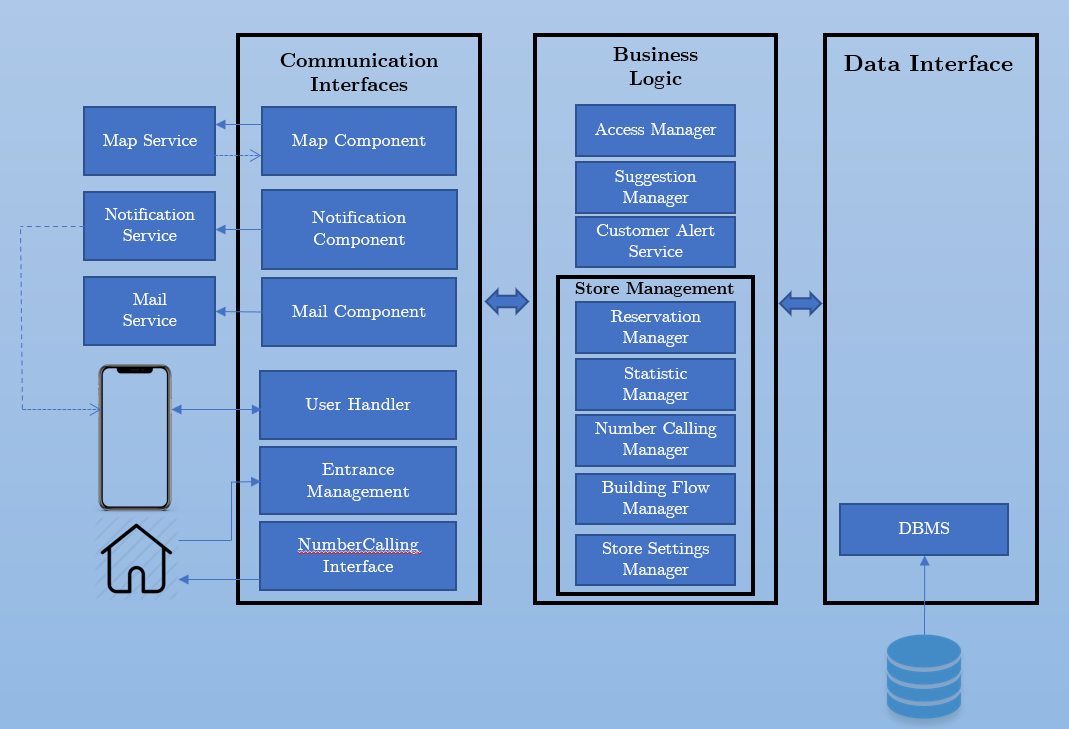
\includegraphics[scale=0.5]{../UML Diagrams/CompositionDiagram/CompositionDiagram.png} \\
		\caption{\emph{Number calling system}}
	\end{figure}
	
		\item{\bfseries Business Logic}: here there is the whole \emph{Business Logic} of the system. Since each store may maintain a different logic from another, there is a \emph{Component} for each store managed by the system. Each store, manages the following aspects:
		\begin{itemize}
			\item{\bfseries Reservation Manager}: manages all the things concerning \emph{reservations} and their making. It's useful also to retrieve some important data, such as ETAs and available time intervals to enter the store;
			\item{\bfseries Statistic Manager}: it's the part used for the calculation of statistics about customers' shopping time, and about the average time spent in a single department. Since each store is different from the other, the statistics are maintained unique per store. This part is also used by \textbf{Reservation Manager} to calculates ETAs and time intervals;
			\item{\bfseries Number Calling System}: is the component dedicated to admit reserved customers inside the store;
			\item{\bfseries Building Flow Manager}: it takes care of processing scanned QR Codes at the entry and the exit of the store;
			\item{\bfseries Store Settings Manager}: manages all the things concerning stores' settings and parameters, such as working hours and capacity (also for each department).
			
		\end{itemize} This subdivision allows to separate better the logic off each store. Moreover, there are component common to each store, so the ones deputy to allow users to request services to the system.
		\begin{itemize}
			\item {\bfseries Access Manager}: manages users' \emph{registraion} and \emph{log-in};
			\item {\bfseries Suggestion Manager}: manages the retrieve of \emph{suggestions} when required, or necessary;
			\item{\bfseries Customer Alert Service}: takes care of sending departing notifications to customers.
		\end{itemize}
	At the end, there is another block: the \textbf{Data Interface}: it represents the \emph{Data Tier} of the system and separates the Business Logic from the data. It interacts with the DBMS to store and load informations.
	\end{itemize}

	
	\subsection{Component View}
	\subsection{Deployment View}
	\subsection{Runtime View}
	\subsection{Component Interfaces}
	\subsection{Selected Architectural Styles and Patterns}
	\subsection{Other design decisions}

\section{User Interface Design}

\section{Requirements Tracebility}

\section{Implementation, Integration and Test Plan}

\section{Effort Spent}

\section{References}
\end{document}